\chapter{Implementation, Integration \& Testing Plan}

\section{Overview}
This section describes the Implementation, Integration, and Test Plan for the BBP application. The aim is to ensure that the system is built incrementally, with a focus on reliability, modularity, and ease of testing.

The implementation and integration of the BBP application will adopt a Bottom-Up strategy. This approach begins from the components located at the lower levels of the uses hierarchy and proceeds upward to compose complete subsystems and finally the full system. Each module is first verified through unit tests and test drivers (temporary components that invoke and validate the module behavior). Once stable, modules are integrated by replacing drivers with the real dependent components, progressively building larger subsystems until the system-level behavior is achieved. This strategy will ensure that the core data management and business logic services (Application Layer) are stable and reliable before they are exposed through the API Gateway to the Mobile Application (Presentation Layer).


\section{Implementation Plan}
The implementation is organized into sequential phases. Because the backend is decomposed into independently deployable microservices, many components can be developed in parallel once the shared foundations are defined.

The following order guarantees that higher-level components are integrated only when their dependencies have already been validated, which is the core rationale of the bottom-up strategy.

\subsection{Phase 0 - Shared Foundations and Infrastructure}
The goal of this phase is to implement the shared infrastructure required to enable parallel development, ensuring that work proceeds independently yet consistently.

\begin{itemize}
    \item \textbf{Development environment:} set up the source code repository structure and container orchestration configuration (e.g., docker-compose or Kubernetes manifests). This enables developers to launch the complete system infrastructure (databases, message broker, and mock servers) on their local machines with a single command.
    
    \item \textbf{Shared contract libraries:} Implement a common library (e.g., a shared JAR or package) containing the standard API DTOs, Error Codes, and Event Schemas. This ensures that the contracts defined in the design are strictly enforced in code and that all microservices import the exact same data structures.
    
    \item \textbf{Database initialization scripts:} Write and commit the DDL (Data Definition Language) or migration scripts (e.g., Flyway/Liquibase) for AuthDB, TripDB, and PathDB. This ensures that the schemas and indexes are automatically provisioned when the development environment starts.
    
    \item \textbf{Integration test utilities:} Implement the ``Test Utilities'' module, which includes:
    \begin{itemize}
        \item \textbf{Mock Servers:} A configurable HTTP server to stub Map and Weather API responses (handling success, timeout, and failure scenarios).
        \item \textbf{Event Bus Probe:} A utility to inject test events and assert their presence/ordering in the broker, used later to verify asynchronous flows.
    \end{itemize}
\end{itemize}

\subsection{Phase 1 - Data Layer Modules}
The goal of this phase is to implement and test the data persistence layer in isolation, with no external service dependencies.

\begin{enumerate}
    \item \textbf{AuthDB access module:} implement CRUD operations for users (insert, retrieve, update, delete)
    
    \item \textbf{TripDB access module:}
    \begin{itemize}
        \item create trip entry/session
        \item persist sensor batches (time-series)
        \item store/retrieve trip info and trip list
        \item manage status (e.g., pending obstacle)
        \item append-only PublicationLog
    \end{itemize}
    
    \item \textbf{PathDB access module:}
    \begin{itemize}
        \item store/update/retrieve paths and ranking data
    \end{itemize}
\end{enumerate}

\textbf{Drivers:} create ``DB-only Drivers'' that call these interfaces directly to validate constraints and invariants (e.g., assuring PublicationLog immutability).

\begin{figure}[H]
    \centering
    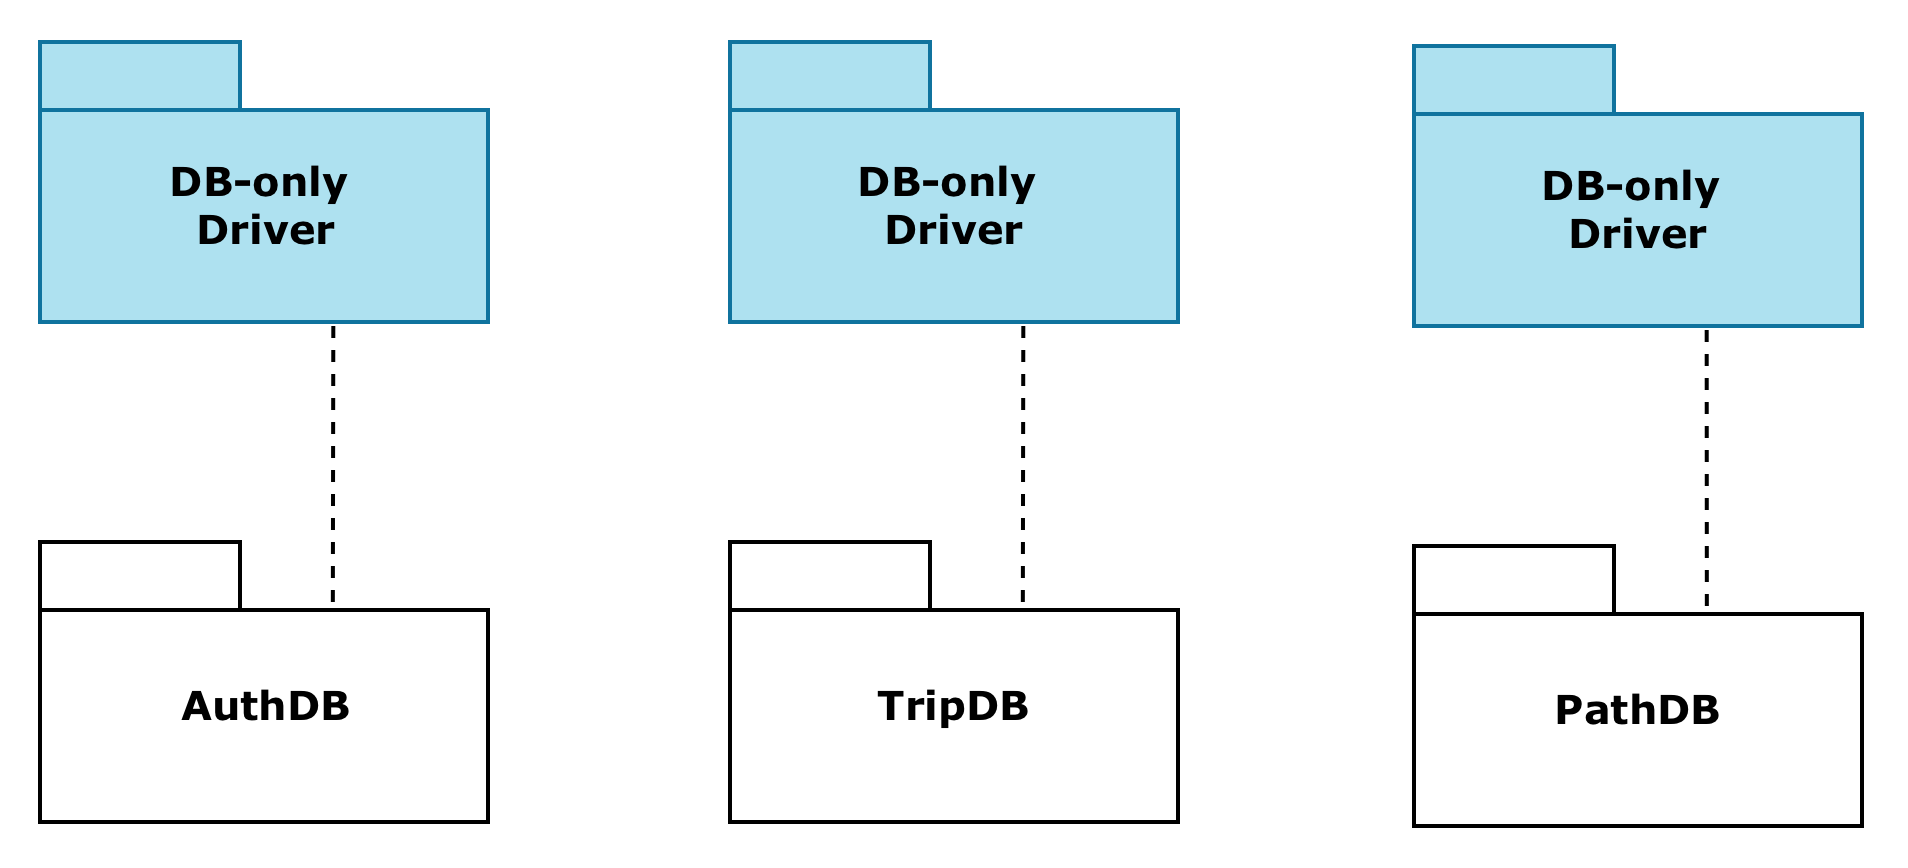
\includegraphics[width=0.8\textwidth]{images/ImplementationPlan_Phase_1.png}
    \caption{Phase 1 - Data Layer Modules}
    \label{fig:phase1_data_layer}
\end{figure}

\subsection{Phase 2 - Message Broker Baseline (Event Bus)}
The goal of this phase is to ensure the asynchronous communication backbone (Pub/Sub) works before connecting business logic.

\begin{itemize}
    \item Configure publisher and consumer groups.
    \item Implement producer/consumer wrappers matching the ``produce(Event, Metadata)'' and ``consume(Event)'' interface.
    \item Contract tests: validate schema enforcement, metadata optionality and idempotency keys.
\end{itemize}

\textbf{Driver:} create publisher/consumer test programs that inject events and verify delivery expectations at application level.

\begin{figure}[H]
    \centering
    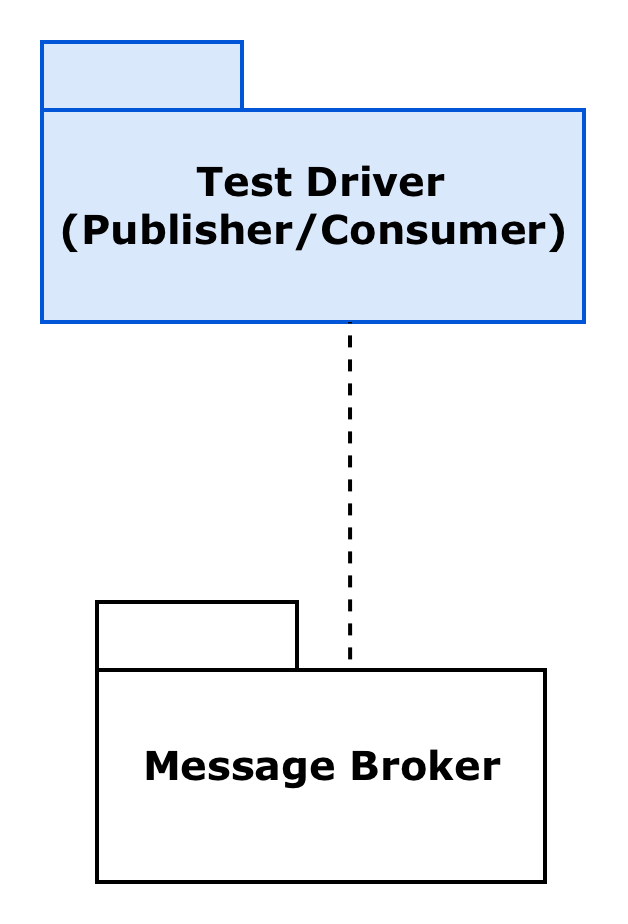
\includegraphics[width=0.3\textwidth]{images/ImplementationPlan_Phase_2.png}
    \caption{Phase 2 - Message Broker Baseline}
    \label{fig:phase2_message_broker}
\end{figure}

\subsection{Phase 3 - Backend Microservices (Business Logic)}
The goal of this phase is to implement services bottom-up, starting from those that create data and moving to those that consume it.

The implementation is split into two sub-stages to maximize parallel development efficiency.

\subsubsection{Stage 1 - Independent Core Services}
These services (Authentication, Trip and Path) can be implemented simultaneously as they primarily depend on their own isolated databases (implemented in Phase 1) and the stable Message Broker (Phase 2).

\begin{enumerate}
    \item \textbf{Authentication Service:} it implements signup/login/JWT issuance and validation. It depends solely on AuthDB and is immediately testable.
    
    \item \textbf{Trip Service:} it owns TripDB and implements trip recording and management logic. It publishes \texttt{AutomaticTripRecorded}, \texttt{ManualTripCreated}, \texttt{TripPublished}, and consumes \texttt{AnalysisCompleted}.
    
    \textit{Note 1:} Since the Analysis Service does not exist yet, a Test Driver injects synthetic \texttt{AnalysisCompleted} events to verify the Trip Service's reaction logic.
    
    \textit{Note 2:} During this phase, interactions with Map Service are simulated using Mock Adapters (defined in Phase 0) to isolate logic testing.
    
    \item \textbf{Path Service:} it owns PathDB and implements path search and visualization.
    
    \textit{Note 1:} Since the Merge Service does not exist yet, a Test Driver injects synthetic \texttt{MergeCompleted} events to verify that the Path Service correctly updates PathDB.
    
    \textit{Note 2:} During this phase, interactions with Map and Weather Services are simulated using Mock Adapters to isolate logic testing.
\end{enumerate}

\begin{figure}[H]
    \centering
    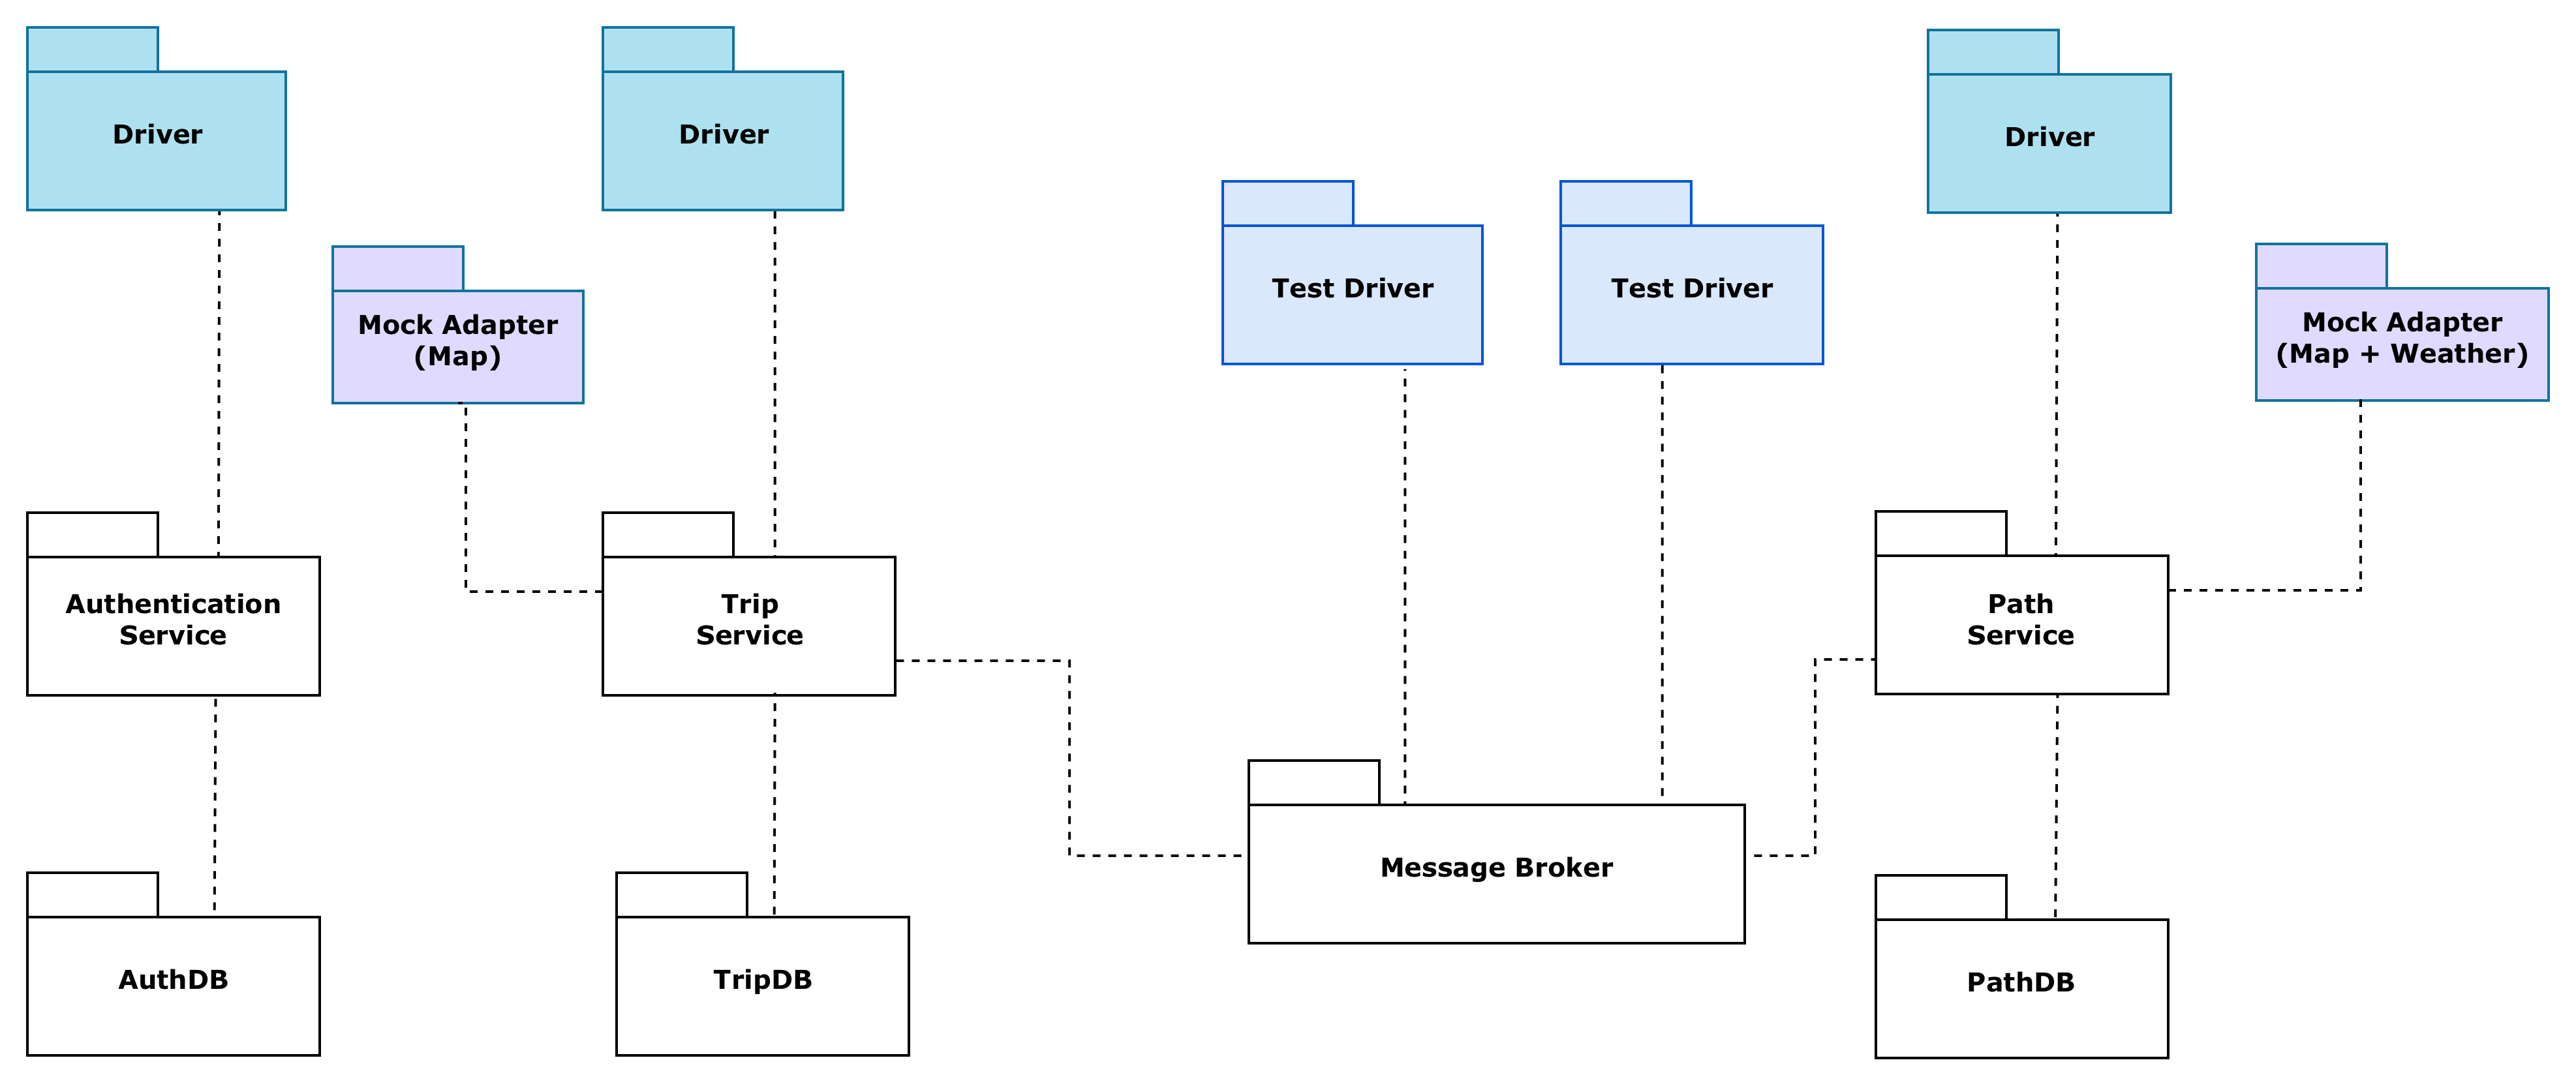
\includegraphics[width=\textwidth]{images/ImplementationPlan_Phase_3_1.png}
    \caption{Phase 3 Stage 1 - Independent Core Services}
    \label{fig:phase3_stage1}
\end{figure}

\subsubsection{Stage 2 - Dependent Services}

\begin{enumerate}
    \setcounter{enumi}{3}
    \item \textbf{Analysis Service:} it depends on Trip Service by consuming \texttt{AutomaticTripRecorded}. It computes statistics, detects anomaly candidates and optionally enriches data with weather information (external Weather Service is simulated using Mock Adapter).
    
    Once analysis is completed, it publishes \texttt{AnalysisCompleted}.
    
    \item \textbf{Merge Service:} it depends on Trip Service by consuming \texttt{TripPublished}. It merges contributions and computes scoring, finally publishing \texttt{MergeCompleted}.
\end{enumerate}

Once the core data producers (Trip Service) are stable, the downstream processing services are implemented and integrated.

\begin{figure}[H]
    \centering
    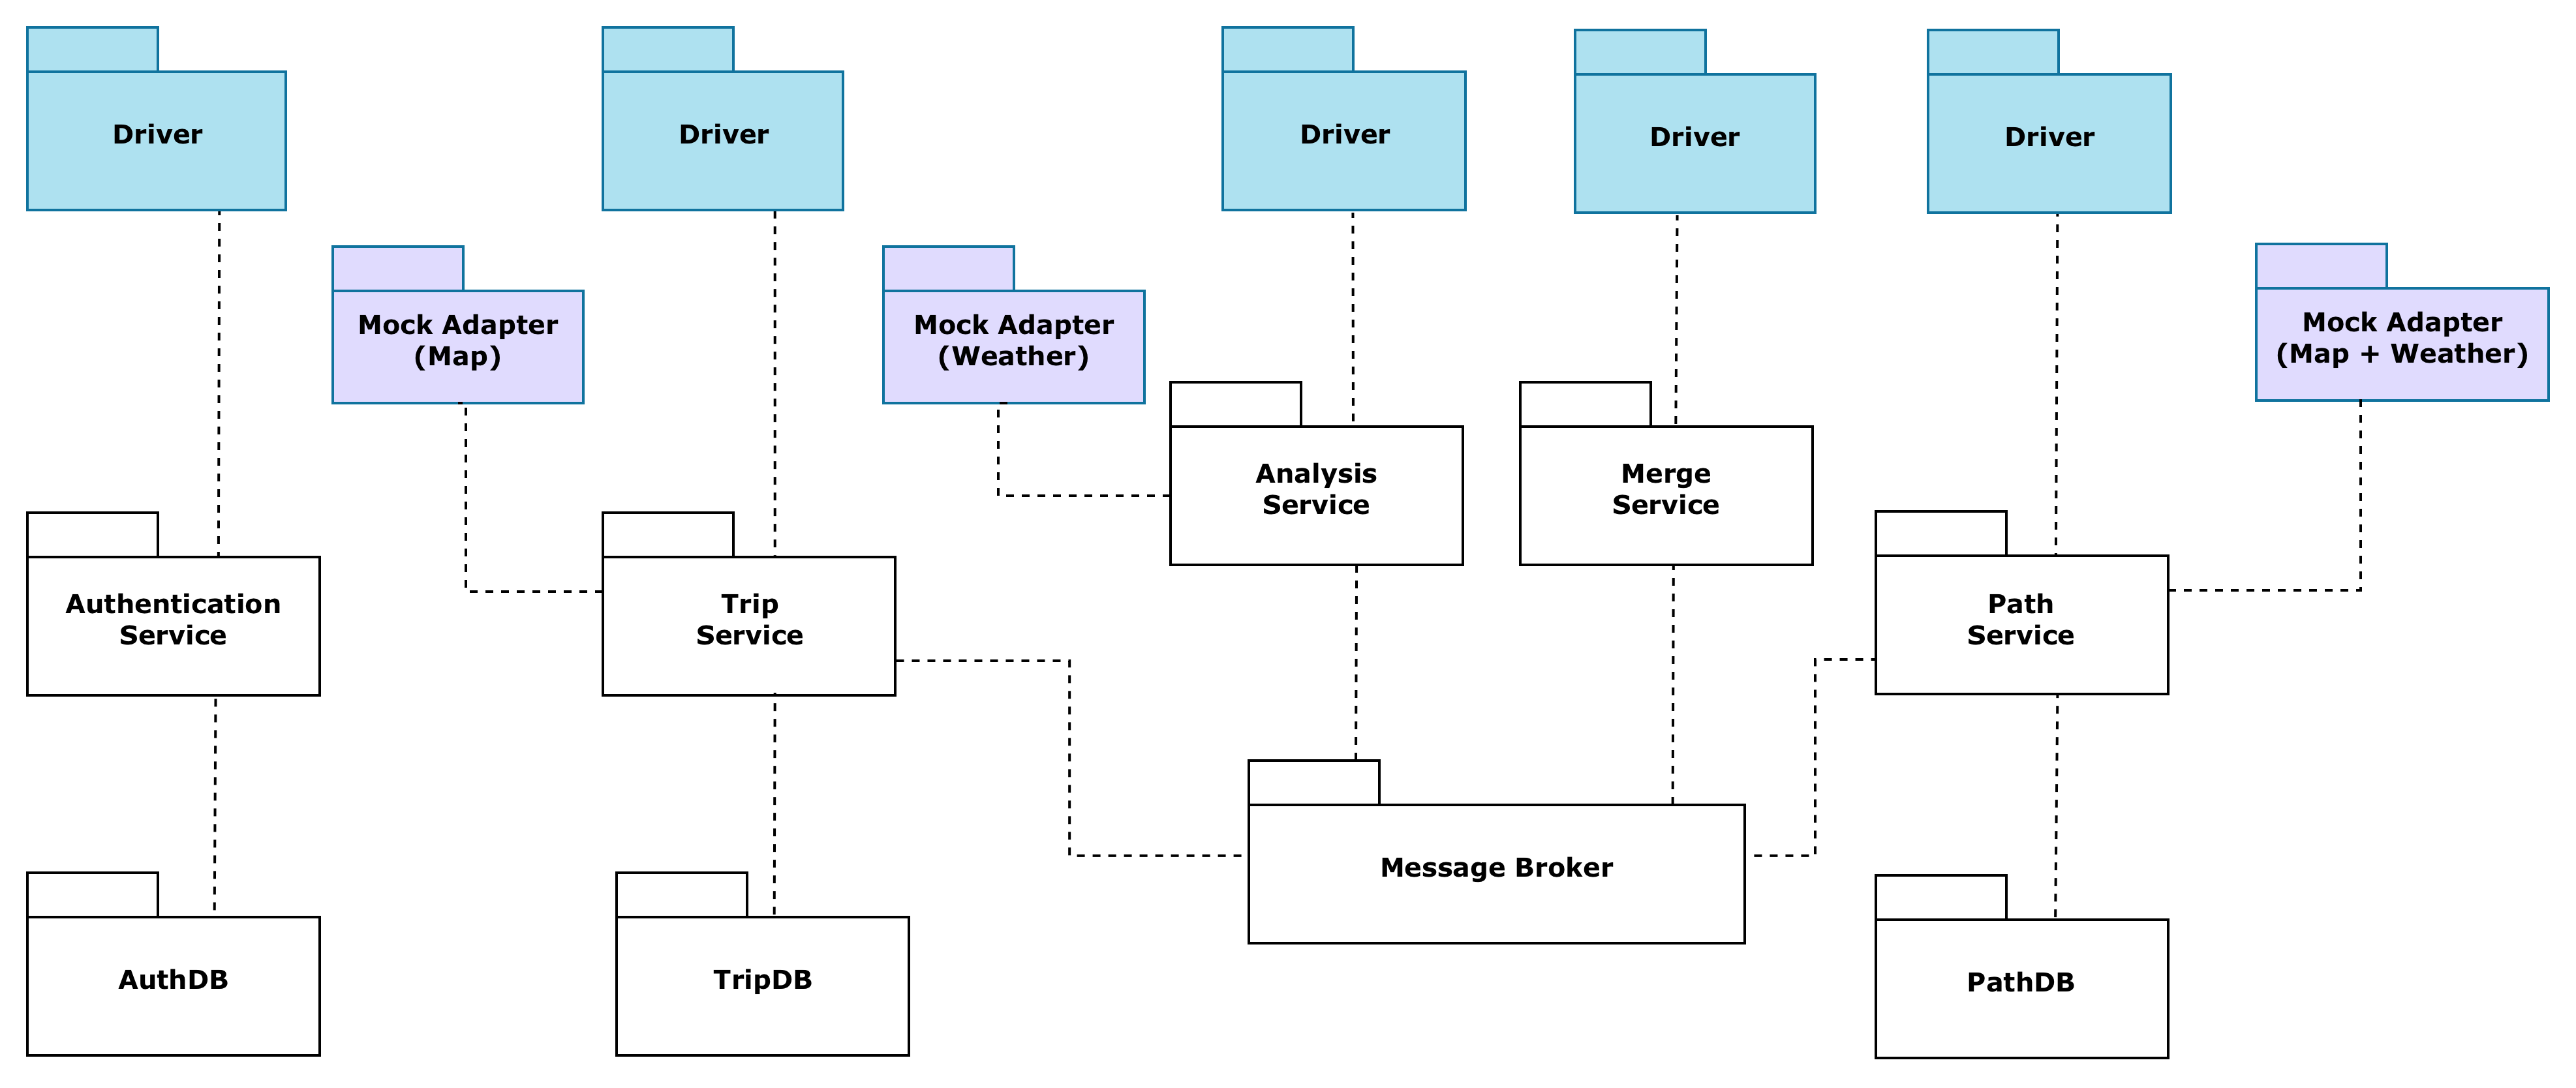
\includegraphics[width=\textwidth]{images/ImplementationPlan_Phase_3_2.png}
    \caption{Phase 3 Stage 2 - Dependent Services}
    \label{fig:phase3_stage2}
\end{figure}

\textbf{Drivers (throughout Phase 3):}
\begin{itemize}
    \item \textbf{REST Drivers} (`Driver' components in the above figures) to call each service interface directly (bypassing API Gateway).
    \item \textbf{Event Drivers} (`Test Driver' components in the above figures) that simulate the missing feedback loops (Analysis/Merge results) until Stage 2 is complete.
\end{itemize}

\subsection{Phase 4 - External Services Integration (Adapters)}
The goal of this phase is to replace the ``Mock Adapters'' with real integrations, stabilizing third-party dependencies before exposing them to end users.

\begin{itemize}
    \item Implement \textbf{Map Service Adapter} and \textbf{Weather Service Adapter} with Circuit Breaker:
    \begin{itemize}
        \item define timeouts, retries policies, open/closed transitions
        \item define fallback behavior (e.g., return cached/partial info or ``weather unavailable'')
    \end{itemize}
    \item Use mock servers to intentionally trigger latency spikes and failures to verify the Circuit Breaker opens and closes correctly.
\end{itemize}

\begin{figure}[H]
    \centering
    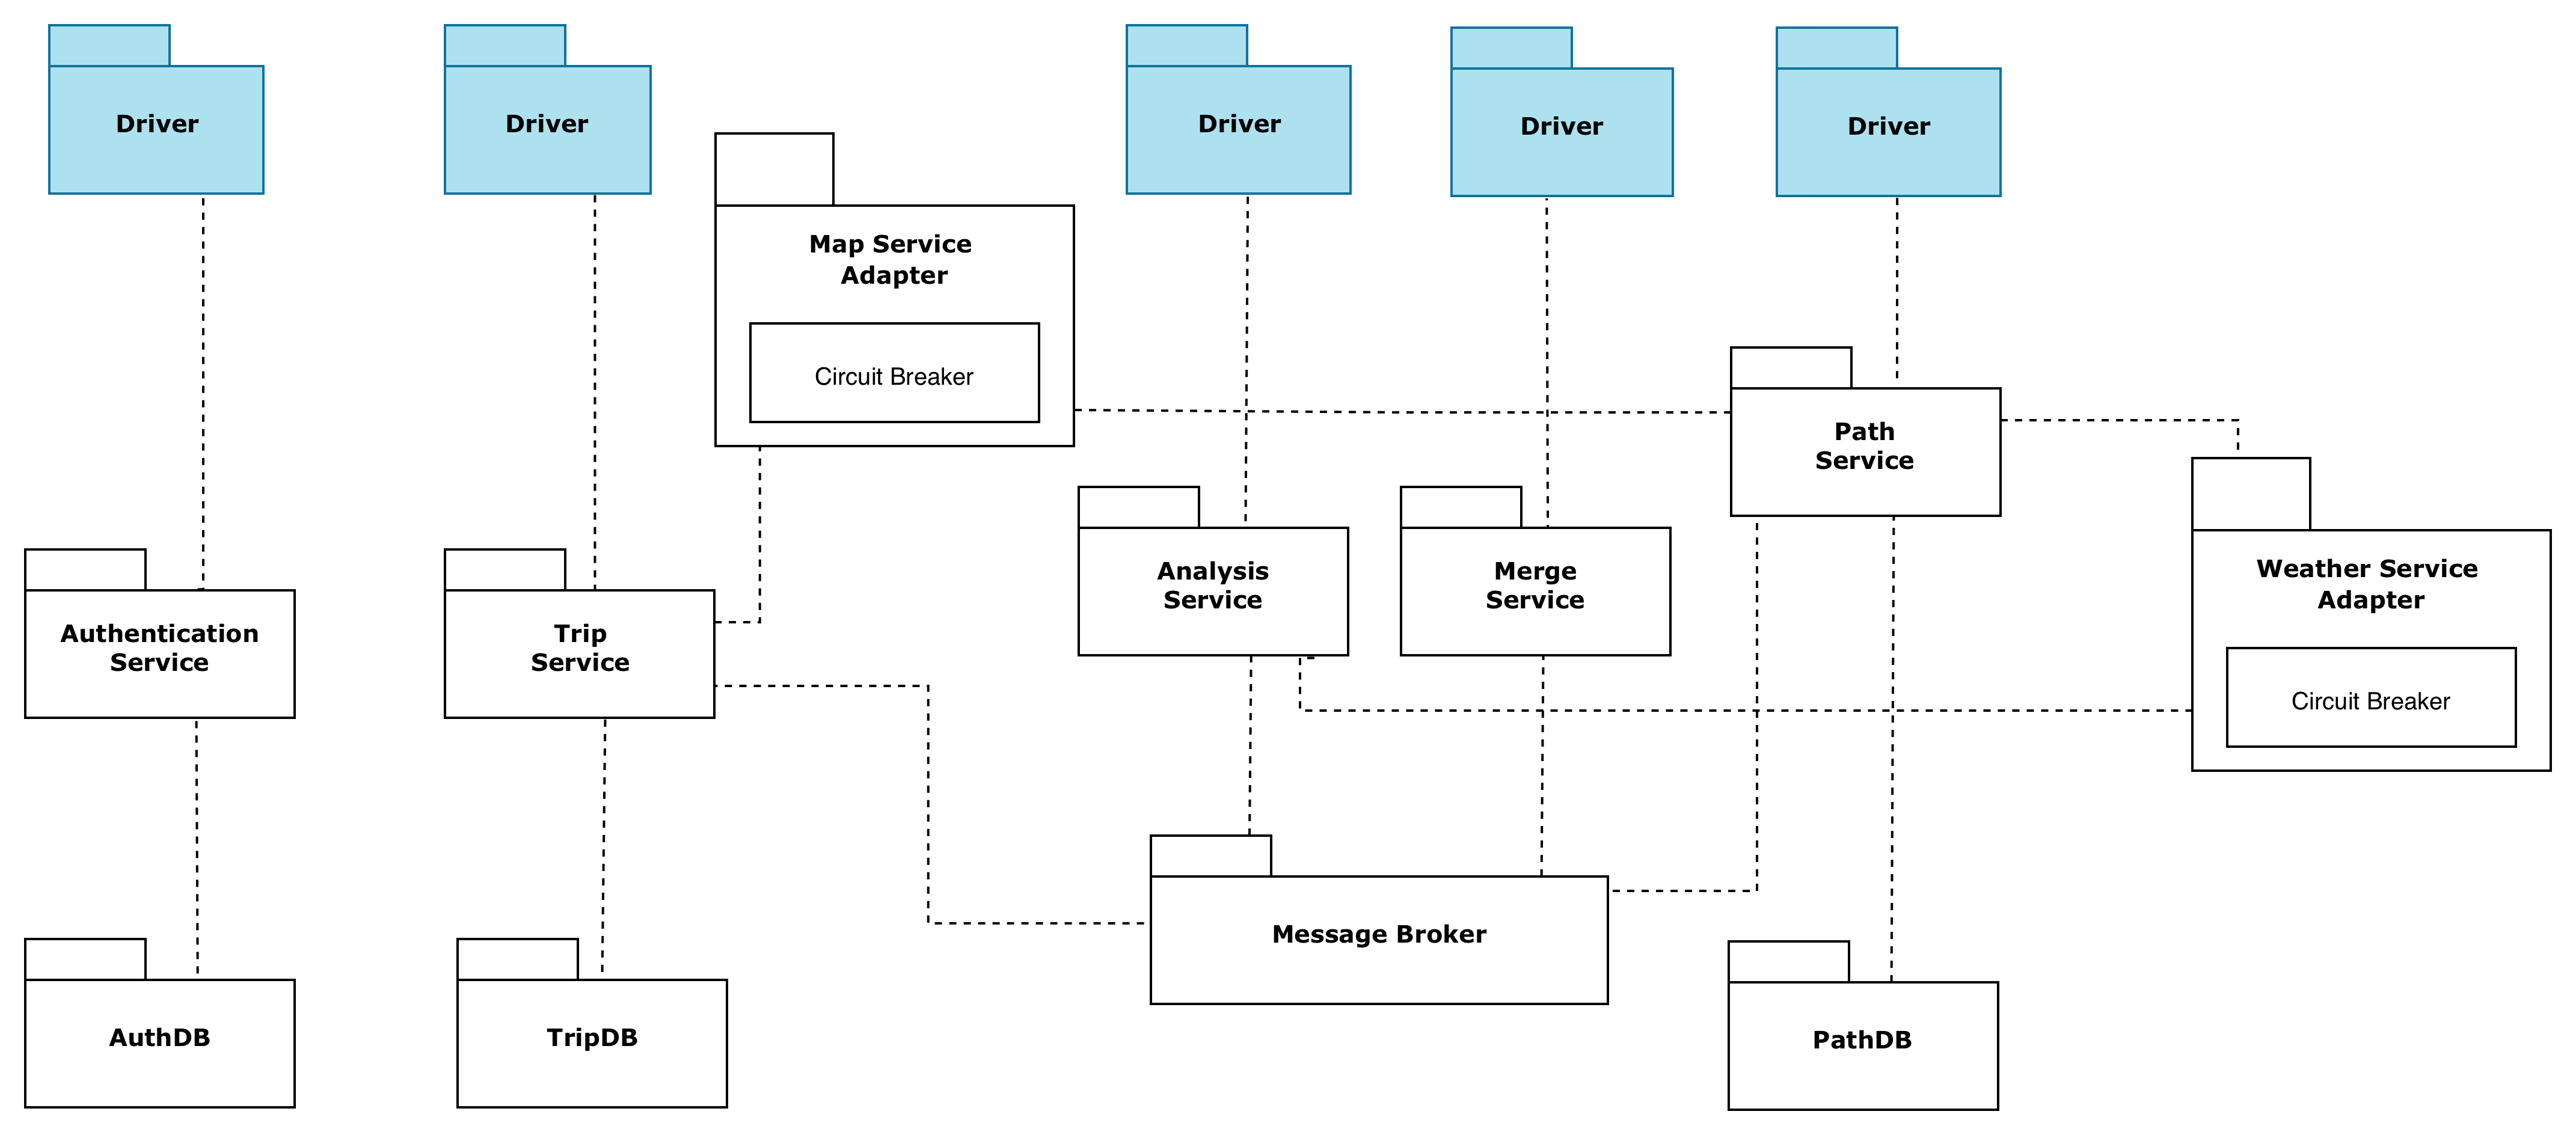
\includegraphics[width=\textwidth]{images/ImplementationPlan_Phase4.png}
    \caption{Phase 4 - External Services Integration}
    \label{fig:phase4_adapters}
\end{figure}

\subsection{Phase 5 - API Gateway}
The goal of this phase is to expose a unified API to the Mobile App only after backend subsystems are stable.

\begin{itemize}
    \item \textbf{Routing:} Implement routing rules to the microservices.
    \item \textbf{Security:} Implement JWT verification, request validation, and TLS termination.
    \item \textbf{Reliability:} Configure rate limiting to protect the backend.
    \item \textbf{Observability:} Add end-to-end request tracing/logging hooks.
\end{itemize}

\subsection{Phase 6 - Mobile App Integration}
The goal of this phase is to connect the User Interface to the now-stable backend endpoints.

\section{System Testing Plan}
Testing is conducted incrementally throughout the development lifecycle, adhering to the Bottom-Up strategy.

\begin{itemize}
    \item \textbf{Unit Testing}
    
    Each subcomponent is tested in isolation, using Mocks and Drivers where needed.
    
    \item \textbf{Integration Testing}
    
    Validate interactions among components by progressively replacing Mocks and Drivers with real dependencies:
    \begin{enumerate}
        \item[(i)] service $\leftrightarrow$ own DB,
        \item[(ii)] service $\leftrightarrow$ message broker,
        \item[(iii)] service $\leftrightarrow$ external providers via adapters (Map/Weather).
    \end{enumerate}
    
    \item \textbf{Functional Testing}
    
    Verify that requirements, use cases and specifications previously described are properly satisfied, by running complete end-to-end scenarios.
    
    \item \textbf{Non-Functional Testing}
    
    Evaluate the system's behavior under high traffic conditions, to identify and address performance bottlenecks. The primary objective is to optimize the application's response time, resource utilization, and throughput, ensuring smooth operation and user satisfaction during peak usage periods.
    
    \begin{itemize}
        \item \textbf{Performance:} API Gateway throughput under concurrent users; ingestion capacity for high-frequency automatic trip data.
        \item \textbf{Security:} JWT enforcement, invalid/expired token handling, request validation and rate limiting effectiveness.
        \item \textbf{Reliability/Fault tolerance \& Recovery:} graceful degradation when Map/Weather is unavailable (circuit breaker), continuity under broker/DB replica failures, and correct restart behavior (durable state preserved, safe re-processing via idempotent consumers).
    \end{itemize}
\end{itemize}
